\chapter[Czym jest bąk? I~cała reszta]{Czym jest bąk? {\red I~cała reszta}\footnote{\red Ten nagłówek pokazuje w~jaki sposób umieścić inną postać tytułu w~nagłówku i~spisie treści (w~spisie np. nieformatowaną). Jeśli potrzebna jest odmienna wersja tekstu w~każdym z~3 miejsc (tytuł rozdziału, spis treści, nagłówek) wówczas należy użyć dodatkowo polecenia \texttt{\textbackslash chaptermark} -- pozwala ono zmienić (np. skrócić jak zrobiono to w~tym przykładzie) treść nagłówków\footnotemark.}\footnotetext{\red Sprawa jest trochę bardziej skomplikowana w~przypadku podrozdziałów -- wówczas należy podać dwukrotnie treść przeznaczoną do nagłówka, według schematu \texttt{\textbackslash section[wersja do spisu treści]\{pełna wersja tytułu\textbackslash sectionmark\{wersja do nagłówka\}\}
\textbackslash sectionmark\{wersja do nagłówka\}}. A~trzeba o~rzecz dbać tylko w~przypadku formatowania tekstu do wydruku dwustronnego, wówczas tytuły podrozdziałów trafiają na nieparzyste strony tekstu.}}
\chaptermark{Czym jest bąk? I~cała\ldots}
\label{czym_jest_bak}

Najprościej rzecz ujmując bąk jest bryłą sztywną zamocowaną [\ldots] a~macierz przejścia z układu ciała do układu przestrzeni ma postać
\begin{equation} \label{equ:macierz_rotacji}
    \RR(\qq) = 
    \resizebox{0.8\hsize}{!}{
    $\begin{bmatrix} 
        \cos \alpha  \cos \gamma -\cos \beta  \sin \alpha  \sin \gamma  & -\cos \beta  \cos \gamma  \sin \alpha -\cos \alpha  \sin \gamma  & \sin \alpha  \sin \beta  \\
        \cos \gamma  \sin \alpha +\cos \alpha  \cos \beta  \sin \gamma  & \cos \alpha  \cos \beta  \cos \gamma -\sin \alpha  \sin \gamma  & -\cos \alpha  \sin \beta  \\
         \sin \beta  \sin \gamma  & \cos \gamma  \sin \beta  & \cos \beta  
    \end{bmatrix}$}
\end{equation}

{\red
  W~przypadku dużych macierzy, długich równań można próbować poradzić sobie z~ich zmieszczeniem przez użycie polecenia \texttt{\textbackslash resizebox} (jak zrobiono to w~równaniu powyżej dla zawartej w~nim macierzy)\footnote{\red Alternatywnie poleceniem\texttt{\textbackslash scalebox} pozwalającym określić docelowy wymiar obiektu w~odniesieniu do jego pierwotnego wymiaru (\texttt{\textbackslash resizebox} pozwala określić wymiar docelowy bezwzględnie lub w~odniesieniu do ,,zewnętrznych obiektów'' -- szerokości tekstu, kolumny itp.).}, lub zmniejszenie używanych w~równaniu czcionek (co poczyniono w~równaniu poniżej, mimo że w~sumie nie było to konieczne:).}

\noindent
[\ldots]

\noindent
Możemy sprawdzić to dokonując rzutowania, a mianowicie
{\small
  \begin{multline}
    \left(\iner\bdvelo, \ee_3\right) = \left(\iner\bdvelo, \RR^T\ee_z\right) =
    \begin{pmatrix}
    \dot\alpha\sin\beta\sin\gamma + \dot\beta\cos\gamma\\ 
    \dot\alpha\sin\beta\cos\gamma - \dot\beta\sin\gamma \\  
    \dot\alpha\cos\beta + \dot\gamma
    \end{pmatrix}^T 
    \begin{pmatrix}
    \sin\beta\sin\gamma \\ \cos\gamma\sin\beta \\ \cos\beta 
    \end{pmatrix} = \\ = \dot\alpha\left(I_1\sin^2\beta + I_3\cos^2\beta\right) + I_3\dot\gamma\cos\beta
\end{multline}}%

{\red
  Równania zajmujące więcej niż jedną linię wygodnie jest robić z~wykorzystaniem otoczenia \texttt{multline}. Łamania dokonujemy na znakach operacji powtarzając je na końcu i~początku linii w~miejscu łamania\footnote{\red W przypadku łamania na znaku minus na końcu linii w~miejscu łamania dajemy znak plus, a~minus umieszczamy na początku kolejnej linii.}. Inne rodzaje otoczeń matematycznych\footnote{\red dostarczanych przez pakiet \texttt{\textbackslash amsmath}} opisane są w~dokumentacji \cite{amsmath}, w~rozdziale 3. O~macierzach traktuje podrozdział 4.2 tamże.}

\section{Bąki swobodne}

[\ldots]

Fizyczną realizacją bąka Eulera spełniającą przypadek pierwszy jest żyroskop -- ciało sztywne umieszczone w~zawieszeniu Cardana, w~taki sposób, aby środek ciężkości pozostawał nieruchomy -- przedstawiony na rysunku~\ref{fig:Ch1_giro_model} wraz z ilustracją modelu matematycznego, gdzie $R$ oznacza środek ciężkości bąka.  
\begin{figure}[tp]
  \centering
  \def\svgscale{1}
  \subfloat[]{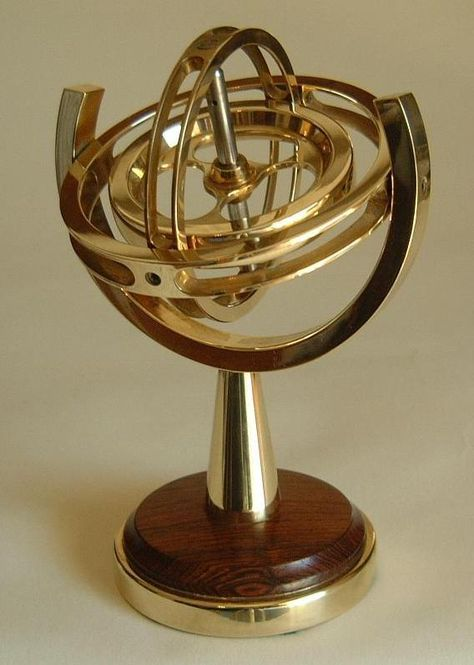
\includegraphics[scale=0.3]{giroskop.jpg}}\hspace{25pt}\qquad
  \subfloat[]{\input{figures/chapter_03/bak_eulera.pdf_tex}}
  \caption{Przykład bąków swobodnych a) żyroskop, \cite{CArn}, b) model bąka Eulera}
  \label{fig:Ch1_giro_model}
    \end{figure}

{\red
  W~przypadku rysunków zawierających kilka części można posłużyć się poleceniem \texttt{\textbackslash subfloat} (zobacz rysunek~\ref{fig:Ch1_giro_model}). Gdy rysunek nie mieści się na jednej stronie, można go podzielić tak, jak to zrobiono w~przypadku rysunku~\ref{fig:portret_fazowy_step} -- użyte mechanizmy dostępne są po dodaniu w~preambule dokumentu pakietu \texttt{subfig}.}
\begin{figure}[tp]
  \centering
  \def\svgscale{0.87}\subfloat[]{\input{figures/chapter_04/elipsoida1a.pdf_tex}}
  \def\svgscale{0.87}\subfloat[]{\input{figures/chapter_04/elipsoida1b.pdf_tex}}\\ 
  \def\svgscale{0.85}\subfloat[]{\input{figures/chapter_04/elipsoida1c.pdf_tex}}
  \def\svgscale{0.85}\subfloat[]{\input{figures/chapter_04/elipsoida1d.pdf_tex}}\\ 
  \def\svgscale{0.83}\subfloat[]{\input{figures/chapter_04/elipsoida1e.pdf_tex}}
  \def\svgscale{0.83}\subfloat[]{\input{figures/chapter_04/elipsoida1f.pdf_tex}}\\ 
  \caption{Kolejne etapy powstawania portretu fazowego (cdn.)}
  \label{fig:portret_fazowy_step}
\end{figure}
\begin{figure}
  \centering
  \ContinuedFloat
  \def\svgscale{0.81}\subfloat[]{\input{figures/chapter_04/elipsoida1g.pdf_tex}}
  \def\svgscale{0.81}\subfloat[]{\input{figures/chapter_04/elipsoida1h.pdf_tex}}\\ 
  \def\svgscale{0.77}\subfloat[]{\input{figures/chapter_04/elipsoida1i.pdf_tex}} 
  \caption{Kolejne etapy powstawania portretu fazowego (cd.)}
\end{figure}

\noindent
[\ldots]

\noindent
Ilustracja opisanej konstrukcji została przedstawiona na rysunku \ref{fig:efekt_poten}. Gdy wykres energii całkowitej nie przecina wykresu $U(\beta)$ oznacza to, że układ taki jest nierealizowany fizycznie jako bąk -- posiada ujemną energię kinetyczną.
\begin{figure}[tp]
    \centering
    \def\svgscale{0.8}
    \input{figures/chapter_04/efektywny_pot.pdf_tex}
    \caption{Wykres efektywnego potencjału}
    \label{fig:efekt_poten}
\end{figure}

\noindent
[\ldots]

\noindent
Gdy $u_L$ zmniejsza się zaczyna formować pętle (rysunek \ref{fig:ul5}).
\begin{figure}[tp]
    \centering
    \subfloat{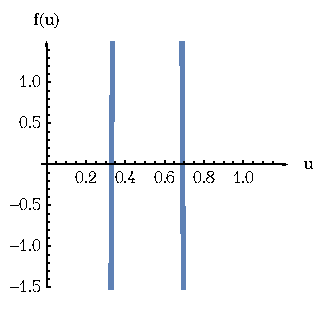
\includegraphics[scale=0.86,valign=m]{figures/chapter_05/ul5_fu.pdf}}
    \subfloat{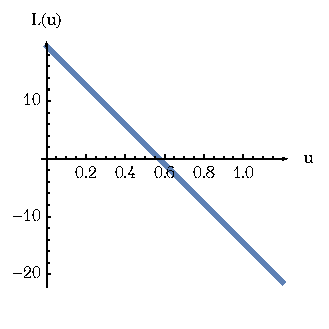
\includegraphics[scale=0.86,valign=m]{figures/chapter_05/ul5_lu.pdf}}
    \subfloat{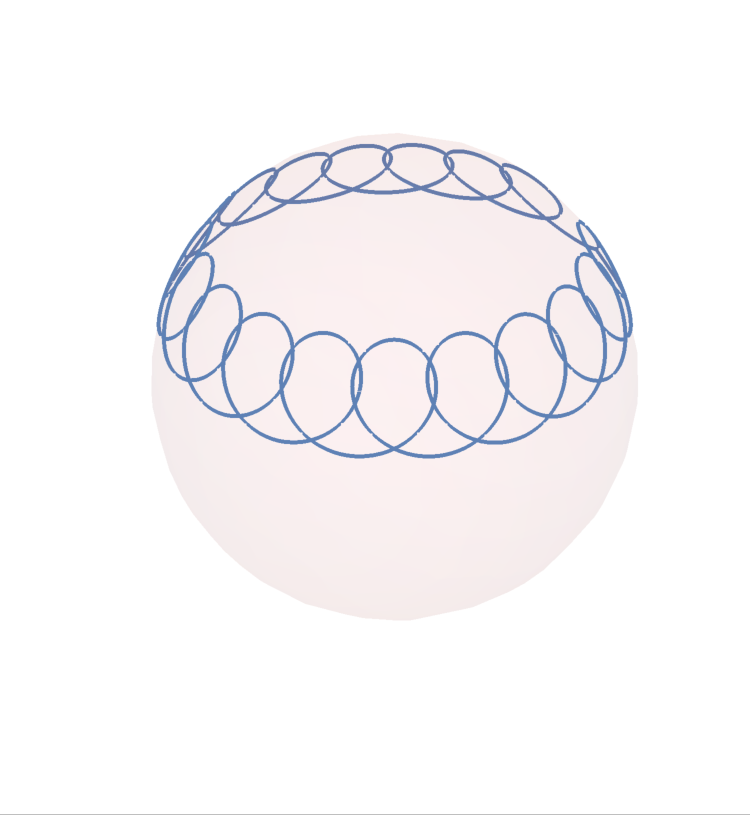
\includegraphics[scale=0.61, trim={1cm 2.5cm 1cm 2.5cm},clip,valign=m]{figures/chapter_05/ul5_trace.pdf}}
    \caption{Przebieg dla $u_1 < u_L < u_2$, $a=114.991$}
    \label{fig:ul5}
\end{figure}

{\red
  Powyższe dwa przykłady (rysunki~\ref{fig:efekt_poten} i~\ref{fig:ul5}) pokazują sposób dołączania wykresów pochodzących z~Inkscape'a i~programu potrafiącego zapisać je w~formacie pdf (Matlab, Mathematica).}

\noindent
[\ldots]

{\red

\section{Inne sprawy}

\subsection{Wykresy, schematy, diagramy, czyli sprawa \texttt{Svg}a i~Ti{\it k}Za}

W~przypadku wykresów i~innych plików, które zostały zapisane w~formacie \texttt{svg} można je dołączyć tak, jak pokazano na rysunku~\ref{fig:svg_input}, na którym to umieszczono wykres wyprodukowany w~środowisku MatLab. 
\begin{figure}[tp]
      \centering
    %\includesvg[scale=0.5, pretex=\scriptsize]{figures/chapter_02/e1_plot_1}
                                          %%w~starszych wersjach pakietu svg nie ma opcji scale :(
    \includesvg[width=0.6\textwidth, pretex=\scriptsize]{e1_plot_1}
    \renewcommand{\figurename}{\red Rysunek}%
    \caption[Wykres uchybu regulacji\ldots]{\red Wykres uchybu regulacji\ldots}
    \label{fig:svg_input}
\end{figure}
Nieco więcej na temat plików \texttt{svg} jest napisane w~komentarzu do rysunku~\ref{fig:transf_se3} na stronie~\pageref{fig:transf_se3}. Alternatywnie wykres można sporządzić korzystając z~pakietu \texttt{pgfplots} \cite{pgfplots} bazującego na języku Ti{\it k}Z. Przykład zaprezentowano na rysunku~\ref{tikz_wykres}.}
\begin{figure}[tp]
  \centering
  \scalebox{0.85}{
    \begin{tikzpicture}
    \begin{axis}[
        title=Kwadratowo,
        xlabel={$x$},
        ylabel={$y$},
      ]
      \addplot table[x expr=\coordindex,y index=0] {figures/chapter_03/data_raw.dat};
    \end{axis}
  \end{tikzpicture}\hspace{5mm}
  \begin{tikzpicture}
    \begin{axis}[
        title=Mój przebieg,
        xlabel={$t$},
        ylabel={$y(t)$},
        grid=major,
      ]
      \addplot [green] table {figures/chapter_03/out.dat};
    \end{axis}
  \end{tikzpicture}}
  \renewcommand{\figurename}{\red Rysunek}%
  \caption[Przykład wizualizacji danych z~pliku]{\red Przykład wizualizacji danych z~pliku}
  \label{tikz_wykres}
\end{figure}

{\red
Jeśli mamy potrzebę przedstawienia prostego schematu blokowego, to może najprościej przygotować go opisując we wspomnianym w~podrozdziale~\ref{narzedzia} języku Ti{\it k}Z, którego tak czy inaczej i~tak warto trochę liznąć. Na rysunkach~\ref{tikz_blok}, \ref{fig:dynamic_lin_diagram} przedstawiono przykłady: pierwszy, prosty, umieszczony w~treści dokumentu i~drugi, bardziej rozbudowany, z~ukazaniem sposobu dołączania z~pliku zewnętrznego\footnote{\red Autor drugiego diagramu bazował na przykładzie \cite{schem_blokowy} i~korzystał z~funkcji \texttt{let} pakietu \texttt{calc}. Po czasie twierdzi, że do przygotowania tak rozbudowanego rysunku użyłby jednak Inkscape'a lub podobnego narzędzia graficznego~\smiley{} Co też w~tym poradniku uczyniono. Po prostu czytaj cierpliwie dalej~\smiley}.}
% zamiast odwołania do rysunku 2.1 wykonać rysunek 3.8 w~Inkscape'ie ale też w~Dia'i
% https://lightonphiri.org/blog/latex-consistent-diagrams-using-dia
%https://en.wikibooks.org/wiki/LaTeX/PGF/TikZ
\begin{figure}[tp]
  \centering
  \scalebox{0.85}{\begin{tikzpicture}[auto, node distance=3.7cm, >=latex]
    
    \node [block] (trajectory) {\makecell{Generator\\trajektorii}};
    \node [sum, right of=trajectory] (sum) {};
    \node [block, right of=sum] (controller) {\makecell{Regulator\\PD}};
    \node [block, right of=controller] (edda) {\makecell{Model\\manipulatora\\EDDA}};
    \node [output, right of=edda] (output) {};
    
    
    \draw [->] (trajectory) -- node {$\mathbf{q_d, \dot{q}_{d}}$} (sum);
    \draw [->] (sum) -- node {$\mathbf{e, \dot{e}}$} (controller);
    \draw [->] (controller) -- node [name=u] {$\mathbf{u}$}(edda);
    \node [output, below of=u, node distance=2cm] (tmp) {};
    
    \draw [->] (edda) -- node [name=y] {$\mathbf{q,\dot{q}}$} (output);
    \draw [->] (y) |- (tmp) -| node[pos=0.99] {$-$} node [near end] {} (sum);
    
      \end{tikzpicture}}
  \renewcommand{\figurename}{\red Rysunek}%
  \caption[Schemat symulowanego układu sterowania dla algorytmu Qu-Dorseya]{\red Schemat symulowanego układu sterowania dla algorytmu Qu-Dorseya}
  \label{tikz_blok}
\end{figure}
\begin{figure}[tp]
  \centering
  \includestandalone[width=0.9\textwidth]{./figures/chapter_02/dynamic-lin}%
  \renewcommand{\figurename}{\red Rysunek}%
  \caption[Dynamic state feedback linearisation \cite{jedrzej}]{\red Dynamic state feedback linearisation \cite{jedrzej}}
    \label{fig:dynamic_lin_diagram}
\end{figure}
{\red Przy opracowywaniu tego typu rysunków można wspomóc się graficznym interfejsem do Ti{\it k}Za o~nazwie TikZiT \cite{tikzit} lub po prostu skorzystać z~Inkscape'a czy podobnego narzędzia, jak opisano to w~punkcie~\ref{grafika_narzedzia} podrozdziału~\ref{narzedzia}. Tutaj, dla przykładu, na rysunku~\ref{fig:dynamic_lin_diagram_ink} pokazano ten sam diagram co na rysunku~\ref{fig:dynamic_lin_diagram} przygotowany właśnie z~użyciem Inkscape'a\footnote{\red Diagramy nie są idealnie identyczne -- niestety opracowując w~Inkscape'ie grafikę w~której zostaną użyte te same czcionki co w~tekście wszystkie napisy trzeba pozycjonować ręcznie, co w~przypadku Ti{\it k}Za dzięki użyciu pakietu \texttt{calc} odbywa się automatycznie\footnotemark. Ci co zajrzeli do pliku źródłowego \texttt{dynamic-lin\_ink.svg}\footnotemark{} wiedzą o~co chodzi \smiley{}  Inny przykład inkscape'owego rysunku pokazano na stronie~\pageref{fig:transf_se3}.}\addtocounter{footnote}{-1}\footnotetext{\red No prawie zawsze \smiley}\addtocounter{footnote}{1}\footnotetext{\red Oczywiście przy użyciu programu Inkscape \smiley}.
\begin{figure} [tp]
  \centering%
  \scalebox{1.0}{\def\svgwidth{0.9\textwidth}
    \input{figures/chapter_02/dynamic-lin_ink.pdf_tex}}
  \renewcommand{\figurename}{\red Rysunek}%
  \caption[Dynamic state feedback linearisation from Inkscape \cite{jedrzej}]{\red Dynamic state feedback linearisation from Inkscape \cite{jedrzej}}
    \label{fig:dynamic_lin_diagram_ink}
\end{figure}
Podobnie można postąpić, gdy potrzebujemy przygotować jakiś diagram przepływu danych czy też diagram algorytmu, choć tu prymarnym wyborem może się okazać program Dia\todo{Dodać przykład w~Dia \cite{dia_fonty}} \cite{dia,dia_wiki}.

  
\subsection{Kod źródłowy, pseudokod, czyli trudna sprawa}

W~zasadzie wydaje się, że wystarczyłoby napisać, iż do umieszczania w~dokumentach kodu źródłowego służy pakiet \texttt{listings}. Jednakże w~podstawowej wersji zapewniane przez niego formatowanie jest bardzo ubogie, co zazwyczaj prowadzi do potrzeby jego konfigurowania. Przykłady jak to zrobić można znaleźć na stronie \cite{list_wiki} czy w~dokumentach opisujących użycie tego pakietu. Alternatywę dla pakietu \texttt{listings} stanowi ostatnio coraz popularniejszy pakiet \texttt{minted}\footnote{\red Jednakże korzystanie z~tego pakietu wymaga zainstalowania kompilatora Phytona oraz systemu podświetlania składni Pygments, zaś sam kompilator pdflatecha musi być wywoływany z~dodatkową opcją \texttt{--shell-escape}.}, z~którego skorzystamy w~poniższych przykładach. Zanim jednak pojawią się przykłady, kilka słów wyjaśnienia, czemu sprawa jest trudna.

Zasadniczo, trudno jest wskazać jedno, uniwersalne rozwiązanie wygodne do przytaczania fragmentów programów, algorytmów zapisanych w~pseudokodzie. Mo\-żna je chociażby umieszczać bezpośrednio w~tekście, jako obiekty pływające w~postaci rysunków, czy też jako obiekty pływające utworzone niezależnie od rysunków. Co lepiej zapewne zależy od tego, czy w~pracy będziemy mieli mnóstwo takich wydruków, czy tylko kilka, czy będą długie, czy krótkie, czy towarzyszyć im będzie dużo tekstu, czy niewiele. Sprawa dodatkowo komplikuje się, jeśli nasze wydruki nie będą mieścić się na pojedynczej stronie i~trzeba będzie je umieszczać jako obiekty wielostronicowe. A~do tego trzeba zadbać o~prawidłowe kodowanie narodowych liter diakrytyzowanych, jeśli takowe w~dołączanych wydrukach występują\footnote{\red Nie wszystkie kroje czcionek używane typowo do składu wydruków zawierają inne, niż podstawowe znaki diakrytyczne.}. Tak czy inaczej, by nie mieć z~kodem źródłowym problemów warto rzecz przemyśleć już na początku pracy z~dokumentem, wybrać jedno, dwa środowiska, naszym zdaniem wygodne w~danej sytuacji i~trzymać się przyjętego rozwiązania.

By przytoczyć wydruk programu bezpośrednio w~tekście wystarczy użyć otoczenia \texttt{minted}
  \begin{minted}[bgcolor=OurListingBackground,linenos=true]{c}
    int pow3(int x) {
      return x * x * x;
    }

    int a = 2, b = 3;
    int y = pow3(a) + b;
    int z = a + pow3(y);
  \end{minted}
W~typowych instalacjach takie rozwiązanie pozwala na podświetlanie wydruków z~ponad 300 języków programowania, na używanie styli\footnote{\red polecenie \texttt{\textbackslash usemintedstyle} -- odkomentuj w~preambule tego dokumentu, by zobaczyć efekt} a~także umieszczanie odpowiednio podświetlonych fragmentów kodu \mintinline{python}{print(x**2)} w~tekście.

Jeśli decydujemy się na umieszczanie wydruków w~sposób wystawiony, możemy do tego celu użyć po prostu otoczenia \texttt{figure}\footnote{\red Co wydaje się rozsądne, gdy w~naszym tekście jest niedużo tak sformatowanych wydruków -- będą one numerowane jednolicie z~rysunkami i~będziemy mówić po prostu, że dany wydruk jest umieszczony na rysunku~\ref{rys:wyd}.}
\begin{figure}[tp]
    \begin{minted}[frame=single,framesep=10pt,fontsize=\scriptsize]{c}
void full_2_cse_static_lin_eta(float eta[5], const float u[5], const float q[9])
{
    float x0 = q[4];
    float x1 = q[2];
    float x2 = sinf(x1);
    float x3 = 1.0F/R;
    float x4 = u[0]*x3;
    float x5 = cosf(x1);
    float x6 = u[1]*x3;
    float x7 = q[3];
    float x8 = 1.0F/cosf(x7);
    float x9 = x4*x5;

    eta[0] = -u[3]*sinf(x0) + x2*x4 - x5*x6;
    eta[1] = u[3]*cosf(x0)*tanf(x7) + x10*x8 + x8*x9;
    eta[2] = u[3];
}
    \end{minted}
  \renewcommand{\figurename}{\red Rysunek}%
  \caption[Przykładowy wydruk umieszczony na rysunku]{\red Przykładowy wydruk umieszczony na rysunku}
    \label{rys:wyd}
\end{figure}
lub dostarczonego przez pakiet \texttt{minted} otoczenia \texttt{listing}, co spowoduje, że wydruki programów będą numerowane niezależnie i~nazywane wydrukami, jak ten pokazany na wydruku~\ref{lst:example}.
\begin{listing}[tp]
    \begin{minted}[frame=single,framesep=10pt,fontsize=\scriptsize]{c}
void full_2_cse_static_lin_eta(float eta[5], const float u[5], const float q[9])
{
    float x0 = q[4];
    float x1 = q[2];
    float x2 = sinf(x1);
    float x3 = 1.0F/R;
    float x4 = u[0]*x3;
    float x5 = cosf(x1);
    float x6 = u[1]*x3;
    float x7 = q[3];
    float x8 = 1.0F/cosf(x7);
    float x9 = x4*x5;

    eta[0] = -u[3]*sinf(x0) + x2*x4 - x5*x6;
    eta[1] = u[3]*cosf(x0)*tanf(x7) + x10*x8 + x8*x9;
    eta[2] = u[3];
}
    \end{minted}
\SetupFloatingEnvironment{listing}{name=\red Wydruk}
\caption{\red Przykładowy kod programu}
\label{lst:example}
\end{listing}
Należy jednak pamiętać, że takie formatowanie ogranicza wielkość kodu do pojedynczej strony.

By dowiedzieć się więcej na temat tego, jak automatycznie łamać długie linie w~kodzie programu, jak łamać kod pomiędzy kolejnymi stronami i~tym podobnych spraw, wystarczy zajrzeć do dokumentacji pakietu \texttt{minted} \cite{minted}.}
